% Import required TikZ libraries
\usetikzlibrary{shapes,shadows,arrows}

% Define some reusable styles
\tikzstyle{decision} = [diamond, draw, fill=white]
\tikzstyle{line} = [draw, -stealth, thick]
\tikzstyle{elli}=[draw, ellipse, fill=gray!20, minimum height=8mm, text width=5em, text centered]
\tikzstyle{block} = [draw, rectangle, fill=white, text width=8em, text centered, minimum height=15mm, node distance=10em]

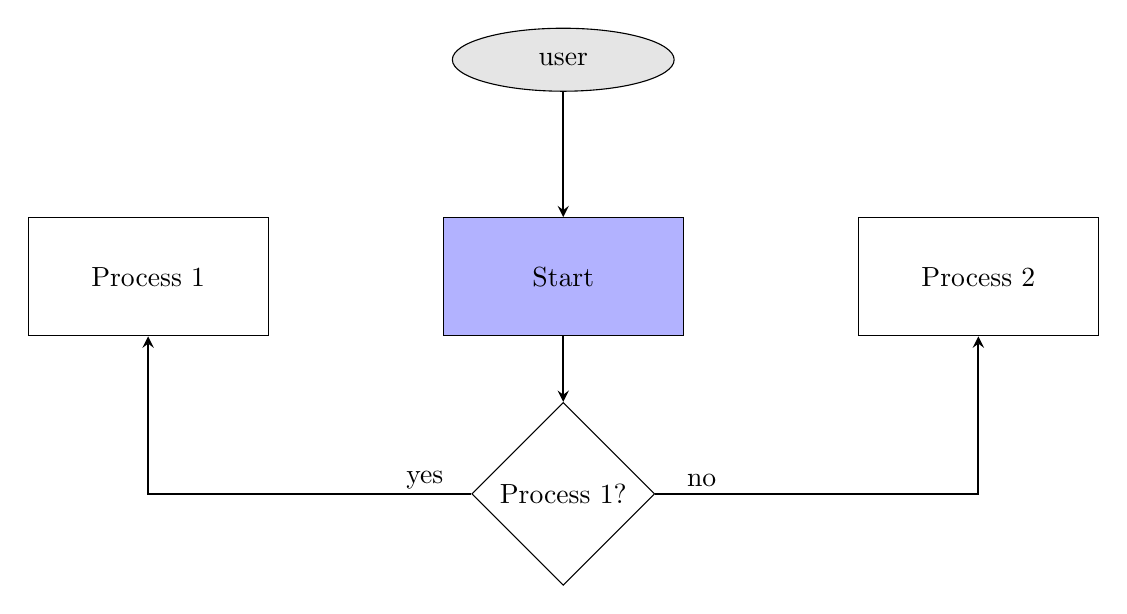
\begin{tikzpicture}
    % Create Blocks
    \node [block,fill=blue!30!white] (start) {Start};
    \node [block, left of=start, xshift=-5em] (process1) {Process 1};
    \node [elli, above of=start, yshift=5em] (user) {user};
    \node [block, right of=start, xshift=5em] (process2) {Process 2};
    \node[decision, below of=start, yshift=-5em](decision1){Process 1?};
    % Add Arrows
    \path [line] (user) -- (start);
    \path [line] (start) -- (decision1);
    \path [line] (decision1) -| node[yshift=0.5em, xshift=10em] {yes} (process1);
    \path [line] (decision1) -| node[yshift=0.5em, xshift=-10em] {no} (process2);
\end{tikzpicture}